\documentclass[11pt]{article}
\newcommand{\blind}{0}



\usepackage[nodisplayskipstretch]{setspace}
\setstretch{1}

\usepackage[utf8]{inputenc}
\usepackage{lipsum}

\usepackage{amsmath,amssymb}
\usepackage{natbib}


\usepackage{amssymb,amsbsy,amsfonts,amsmath,xspace,amsthm}
\usepackage{mathrsfs}
\usepackage{graphicx}


\usepackage{caption}
\usepackage[font=footnotesize]{caption}
\usepackage{setspace}
\usepackage{comment}
\doublespacing
\usepackage[margin=.9in]{geometry}
\usepackage{enumitem} 
\usepackage{subcaption}
\usepackage{multirow}
\usepackage{epstopdf}
\usepackage{epsfig}
\usepackage[colorlinks,citecolor=blue]{hyperref}

\usepackage{url}
\usepackage[toc,page]{appendix}
\usepackage{float}
\usepackage{natbib}
\usepackage{color}
\usepackage[dvipsnames]{xcolor}
\usepackage{verbatim}
\usepackage{authblk}
\usepackage[normalem]{ulem}

\setlength{\textfloatsep}{6pt plus 1.0pt minus 2.0pt}

\def\ack{\section*{Acknowledgements}%
  \addtocontents{toc}{\protect\vspace{6pt}}%
  \addcontentsline{toc}{section}{Acknowledgements}%
}


\usepackage{hyperref}
\hypersetup{
    colorlinks=true,
    linkcolor=blue,
    filecolor=magenta,      
    urlcolor=cyan,
    citecolor=blue
}
 
 


\usepackage{amsmath}
\usepackage{graphicx}
\newcommand*{\KeepStyleUnderBrace}[1]{%f
\mathop{%
\mathchoice
{\underbrace{\displaystyle#1}}%
{\underbrace{\textstyle#1}}%
{\underbrace{\scriptstyle#1}}%
{\underbrace{\scriptscriptstyle#1}}%
}\limits
}
\usepackage{mathtools}
\mathtoolsset{showonlyrefs}
\usepackage{amsmath,amssymb,amsthm,bm,hyperref}
\usepackage{dsfont,listings}

 

\usepackage[ruled,vlined]{algorithm2e}
\SetAlFnt{\small}
\SetAlCapFnt{\small}
\SetAlCapNameFnt{\small}

\usepackage{enumitem}
\theoremstyle{definition}
\newtheorem{schm}{Scheme}
\newtheorem*{schm*}{Scheme}
\newtheorem{thm}{Theorem}[section]
\newtheorem{lem}{Lemma}
\newtheorem{prop}{Proposition}
\newtheorem{property}{Property}
\newtheorem{assumption}{Assumption}

\newtheorem{corollary}{Corollary}[section]
\newtheorem{defn}{Definition}
\newtheorem{example}{Example}
\newtheorem{rmk}{Remark}
\newtheorem{clm}{Claim}

\usepackage{xcolor}
\allowdisplaybreaks
\input macros.tex

\setcounter{secnumdepth}{3}

\def\spacingset#1{\renewcommand{\baselinestretch}%
{#1}\small\normalsize} \spacingset{1}
\def\fixme#1#2{\textbf{\color{red}[FIXME (#1): #2]}}
\def\mycomment#1{\textbf{\color{blue}#1}}
\def\ccomment#1{\textbf{\color{ForestGreen}#1}}
\usepackage{hyperref}
\usepackage[parfill]{parskip}
\usepackage{bm}


\newcommand{\Hnorm}[1]{\left\lVert#1\right\rVert_{\tH_\alpha}}
\newcommand{\nullnorm}[1]{\left\lVert#1\right\rVert}
\def\trueB{\mB^{\text{true}}}
\def\newX{\mX_{\textup{new}}}
\def\newy{y_{\textup{new}}}
\def\sign{\textup{sign}}
\def\bayesf{f_{\textup{bayes}}}
\def\bayesS{S_{\textup{bayes}}}
\def\bayespif{f_{\textup{bayes},\pi}}
\def\CNN{\text{\bf \small CNN }}
\def\Lasso{\text{\bf \small Lasso }}
\def\NonparaM{\text{\bf \small NonMAR }}
\def\LogisticM{\text{\bf \small LogisticM }}
 
 

\usepackage{setspace}
\doublespacing
 
\begin{document}

\if1\blind
{   \date{}
  \title{\vspace*{-2cm}\bf Nonparametric learning with matrix-valued predictors in high dimensions}
\author{\vspace*{-.3cm} Chanwoo Lee$^{1}$, Lexin Li$^2$, Hao Helen Zhang$^3$, and Miaoyan Wang$^1$\\\vspace*{-.2cm}
$^1$Department of Statistics, University of Wisconsin-Madison\\
$^2$Department of Biostatistics and Epidemiology, University of California at Berkeley\\
$^3$Department of Mathematics, University of Arizona\\
}

    \maketitle
} \fi

\if0\blind
{
 \date{}
  \title{\vspace*{-1cm}\bf Nonparametric learning with matrix-valued \\predictors in high dimensions}
\author{}
\maketitle
} \fi

\vspace{-2cm}
\begin{abstract}
We consider the problem of learning the relationship between a binary label response and a high-dimensional matrix-valued predictor. Prediction based on matrices or networks has recently surged in brain connectivity studies, sensor network localization, and integrative genomics. Traditional regression methods take a parametric procedure by imposing a priori functional form between variables. These parametric models, however, are inadequate for structure learning and often fail in accurate prediction. Here, we develop a learning reduction framework to address a range of learning tasks from classification to regression for matrix-valued predictors. Our proposal achieves interpretable prediction via a low-rank two-way sparse representation of the target function. Unlike earlier approaches, our method automatically learns and exploits the important features in the high-dimensional matrices. Statistical accuracy, excess risk bounds, and efficient algorithms are established. We demonstrate the advantage of our method over previous approaches through simulations and applications to human brain connectome data. 

\end{abstract}
\vspace{-.2cm}
\noindent%
{\it Keywords:}  Nonparametric learning, high-dimensional matrices, sparse and low-rank models, classification, regression, feature selection

\vspace{-.3cm}
\section{Introduction }
\vspace{-.5cm}

Matrix-valued predictors ubiquitously arise in modern applications. In brain connectivity studies, for example, individuals are represented by their brain networks, and the networks quantify the connectivity patterns over a set of nodes (brain regions of interest). Human connectom project~\citep{wang2019common} has constructed brain networks for over 1,200 individuals using Desikan atlas with 68 brain nodes. Structural connectivity is measured for every pair of nodes, resulting in an adjacency matrix of size 68 $\times$ 68 for each individual. This connectivity matrix provides important information for disease prediction. Other examples include electroencephalography studies of alcoholism~\citep{zhou2014regularized}. Researchers measure the voltage values from 64 channels of electrodes on 256 subjects for 256 time points. The study yields a $256 \times 64$ matrix-valued feature, along with a binary indicator of subject being alcoholic or not. Identifying the relationship between EEG signals and alcoholism is helpful for disease diagnostics. 


We consider the statistical learning problem of modeling the relationship between a matrix-valued predictor $\mX \in \mathbb{R}^{d_1\times d_2}$ and a binary label response $y\in\{-1,1\}$.  The key challenge with matrix-valued predictors is the high-dimensional multi-way structure in the feature space. One possible approach is to transform the predictors into vectors and apply classical methods such as Lasso \citep{friedman2010regularization}. The practice of vectorization, however, destroys the structural information in the original predictors. Indeed, network data encoded as matrices represent various aspects of features, including global structure (e.g.\ clustering patterns, community hubs) and local structure (e.g.\ node degrees, edge connections). Learning and incorporating these features are important for prediction. There have been several recent attempts to allow matrix-valued predictors; for example, trace regression~\citep{fan2019generalized}, network logistic regression~\citep{relion2019network}, and matrix linear discriminant analysis~\citep{hu2020matrix}. These parametric approaches impose a priori functional form between variables and often lead to inaccurate prediction in high dimensions. For these reasons, nonparametric approaches such as $k$-nearest neighbors, decision trees, and convolutional neural network (CNN) have been popular. Current nonparametric methods aim for accurate prediction at the cost of hard interpretability. In our motivating brain network application and many other scientific studies, however, researchers are interested in {\it interpretable prediction}, where the goal is to not only make accurate prediction but also identify most informative features for descriptive simplicity. Efficient methods that achieve both have yet to be developed. 
 


{\bf Our contributions.} We develop a nonparametric method that automatically exploits the matrix-valued feature space for accurate prediction. We address three matrix problems -- classification, level set estimation, and regression -- via a learning reduction approach. The proposal achieves interpretable prediction using a low-rank two-way sparse representation of the target functions. We establish convergence guarantees in high dimensions that permit the matrix dimension to grow with sample size. Unlike earlier approaches, our method performs efficient variable selection and adapts to the possibly non-smooth, non-linear functions of interest. Our numerical analyses and application demonstrate the outperformance of the proposed approach over previous methods. 


 
{\bf Notation.} Let $\tX=\mathbb{R}^{d_1\times d_2}$ be the feature space. Given a function $f\colon \tX \to \mathbb{R}$, we use $\sign f$ to denote its sign function, such that $\sign f(\mX)=1$ if $f(\mX)>0$ and $\sign f(\mX)=-1$ otherwise. The notion of sign function also extends to sets in $\tX$. We use $\sign (\mX\in A)$ to denote the sign function induced by the set $A\subset\tX$, i.e.,\ a function taking value $1$ on the event $\{\mX\in A\}$ and -1 otherwise. We use shorthand $[n]:=\{1,\ldots,n\}$ to denote the $n$-set for $n\in\mathbb{N}_{+}$ and use $|\cdot|$ to denote the cardinality of sets. Let $\newnormSize{}{\cdot}_p$ denote the vector $p$-norm for $p\geq 0$, and $\FnormSize{}{\cdot}$ be the matrix Frobenious norm. Given a $d_1$-by-$d_2$ matrix $\mB$, we use $\mB_i$ to denote the $i$-th row of $\mB$. The $(p,q)$-norm of a matrix $\mB$ is defined as $\newnormSize{}{\mB}_{p,q}=\newnormSize{}{\mb}_q$, where $\mb=(\newnormSize{}{\mB_1}_p,\ldots,\newnormSize{}{\mB_{d_1}}_p)^T\in\mathbb{R}^{d_1}$ consists of the $p$-norms for each of the rows in $\mB$. In particular, $\newnormSize{}{\mB}_{1,0}=|\{i\in [d_1]\colon \mB_i\neq 0\}|$ denotes the number of non-zero rows in $\mB$. An event $E$ is said to occur ``with high probability'' if $\mathbb{P}(E)$ tends to 1 as the matrix dimension $d_{\min}=\min(d_1,d_2)\to\infty$. We denote $a_n\asymp b_n$ if $\lim_n b_n/a_n\rightarrow c$ for some constant $c>$ and denote $a_n\lesssim b_n$ if $\lim_n b_n/a_n\rightarrow 0.$ We use $\mathds{1}(\cdot)$ to denote the indicator function. 

\vspace{-.3cm}
\section{Three learning problems}
\vspace{-.5cm}

We present the main learning goals of our interest. Let $\mX\in\mathbb{R}^{d_1\times d_2}$ denote the matrix-valued predictor, $y\in\{-1,1\}$ denote the binary label response, and $\mathbb{P}_{\mX,y}$ denote the unknown joint probability distribution over the pair $(\mX,y)$. In the context of binary response, $y$ is a Bernoulli random variable with conditional probability $p(\mX)\stackrel{\text{def}}{=}\mathbb{P}(y=1|\mX)$; we generally make no parametric assumptions on the marginal distribution $\mathbb{P}_{\mX}$ or form of $p(\mX)$. 


Suppose that we observe a sample of $n$ training data points, $(\mX_1,y_1),\ldots,(\mX_n,y_n)$, identically and independently distributed (i.i.d.) according to $\mathbb{P}_{\mX,y}$. Let $(\mX_{\text{new}},y_{\text{new}})$ be a future unseen test point drawn independently from the same distribution. Our goal is to predict $y_{\text{new}}$ based on $\mX_{\text{new}}$. We often omit the subscript ``new'' and simply write $(\mX,y)$ for the prototypical test point. The relevant probabilistic statements should be interpreted as taken jointly with respect to $(\mX,y)$.

We consider three learning problems: classification, level set estimation, and regression. 

\begin{enumerate}[label={2.\arabic*},wide, labelwidth=!, labelindent=0pt]
\item {\it Matrix classification}: Classification is the problem of predicting the label $y\in \{-1,1\}$ to which the new matrix $\mX$ belongs. A prediction rule (also called a classifier) decides that $y=1$ if $\mX\in S$ and $y=0$ if $\mX \not\in S$, where $S$ is a Borel subset of $\mathbb{R}^{d_1\times d_2}$. We formulate the classification problem as choosing a classifier $S\in \tS$, from a given set of candidate classifiers $\tS$, that minimizes the expected classification error 
\begin{equation}\label{eq:classloss}
R(S)=\mathbb{P}_{\mX,y}\left[y\neq \sign(\mX\in S)\right].
\end{equation}
The $R(S)$ is also called the classification risk. When the population distribution $\mathbb{P}_{\mX,y}$ is known, the global minimizer of $R(S)$ over all Borel sets of $\mathbb{R}^{d_1\times d_2}$ is called Bayes classifier, expressed as $\bayesS=\{\mX\in\mathbb{R}^{d_1\times d_2}\colon p(\mX)\geq 1/2\}$. In practice the population distribution is unknown, so the objective function~\eqref{eq:classloss} and the minimizer needs to be estimated through the data $\{\mX_i,y_i\}_{i\in[n]}$. Our first goal is to estimate the Bayes classifier for matrix classification. 

{\bf Question 1.} How to perform classification when matrix dimension far exceeds the sample size $n$?

\item {\it Level set estimation}: The problem of level set estimation generalizes the classification task. For a given $\pi\in(0, 1)$, the target $\pi$-level set of the conditional probability function $p(\mX)$ is defined as
\begin{equation}\label{eq:level}
\bayesS(\pi) = \{\mX\in\mathbb{R}^{d_1\times d_2}\colon p(\mX)\geq \pi\}.
\vspace{-.3cm}
\end{equation}
An important fact is that the set $\bayesS(\pi)$ optimizes the weighted classification risk~\citep{scott2007regression,wang2008probability}. Specifically, among all Borel subsets of $\mathbb{R}^{d_1\times d_2}$, the set $S_{\text{bayes}}(\pi)$ is the global minimizer of the expected $\pi$-weighted classification error,
\begin{equation}\label{eq:risklevel}
R_\pi(S)=\mathbb{E}\left[ w_{\pi}(y)\mathds{1}(y\neq \sign(\mX\in S))\right],
\end{equation}
where we define $w_{\pi}(y)=1-\pi$ or $\pi$ depending on $y=1$ or $-1$. In light of~\eqref{eq:classloss} and~\eqref{eq:risklevel}, the level set estimation is an extension of the usual classification from equal weight $\pi=1/2$ to general weight $\pi \in(0,1)$. Accurate level set estimation plays an important role in applications of geographical elevation maps, imaging contour detection, and motion tracking. We consider the following question:

{\bf Question 2.} How to simultaneously estimate the level set and identify important variables in the matrix-valued predictor space, for the goal of interpretable prediction?


\item {\it Nonparametric regression}: The problem of nonparametric regression is to estimate the conditional mean $\mathbb{E}(y|\mX)$ as a multivariable function in the predictor space. In the our contexts, the nonparametric regression is equivalent to estimating the conditional probability $p(\mX)=\mathbb{P}(y=1|\mX)=\frac{1}{2}(\mathbb{E}(y|\mX)+1)$. Throughout the paper we will focus on $p(\mX)$ and refer to it as the regression function. Our final goal is the function estimation:

{\bf Question 3.} How to learn the regression function $p(\mX)$ in the high-dimensional matrix space?
\end{enumerate}


\begin{figure}\centering
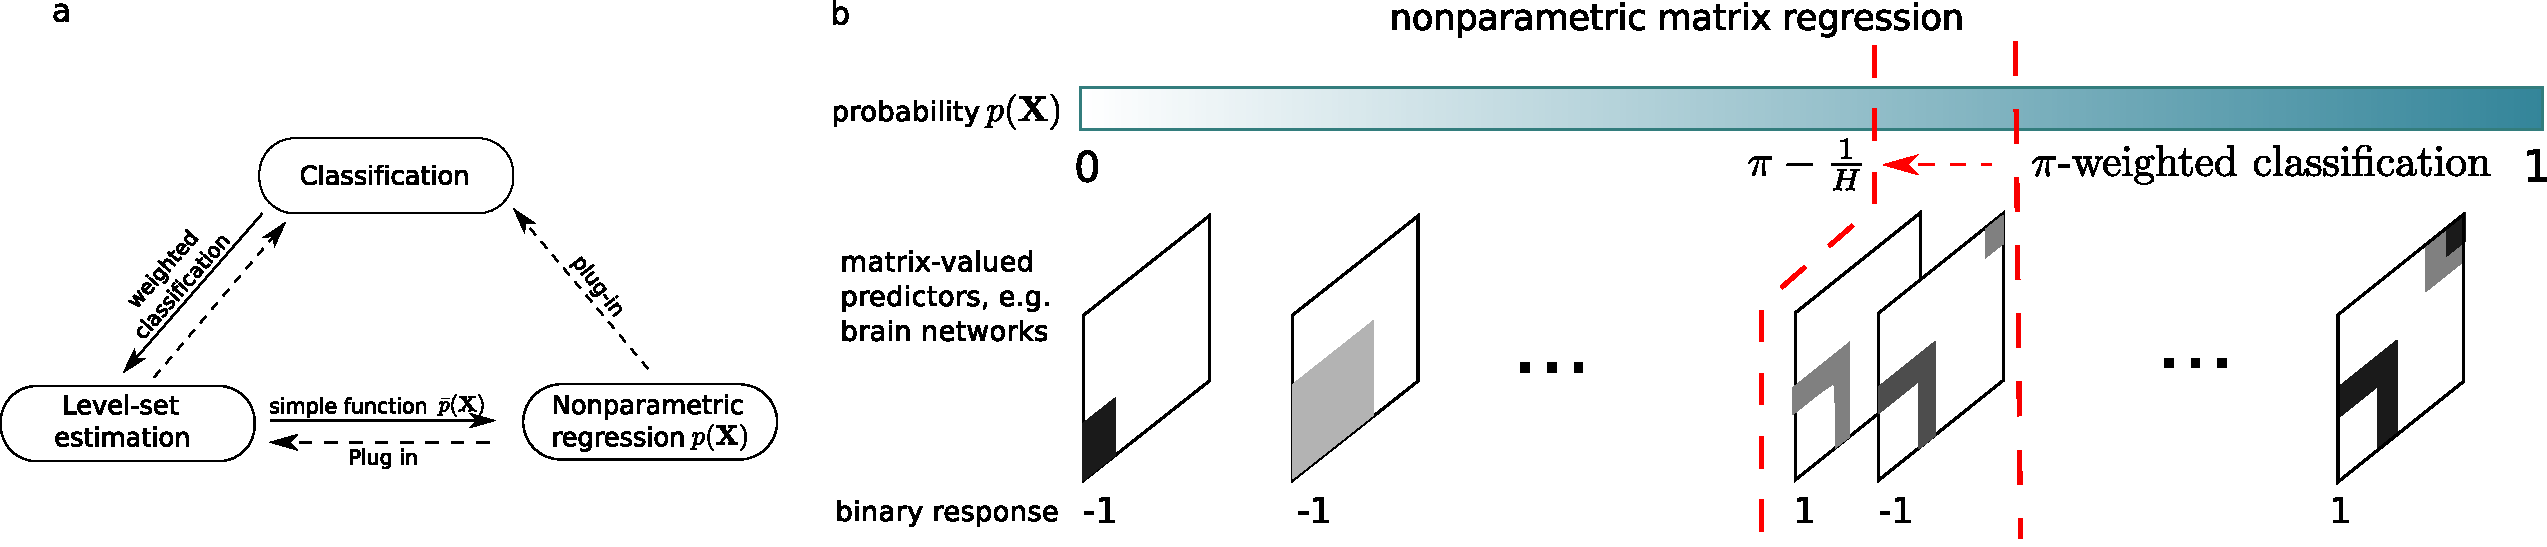
\includegraphics[width=1\textwidth]{new_demo.pdf}
\caption{(a) Our learning reduction approach (solid line) to the three problems of interest. The classical plug-in approaches are depicted in dashed line. (b) Matrix nonparametric regression via $\pi$-weighted classification.}\label{fig:diagram}
\end{figure}

The three problems of our interest represent a range of learning tasks with increasing difficulties. Classification is a special case of level set estimation with $\pi=1/2$, whereas the level set is a discrete approximation of the regression function. A common approach is to address regression first, and then solve the earlier two using plug-in estimates (Figure~\ref{fig:diagram}a). This procedure, however, undermines the fact that regression is generally harder than the other two. Indeed, as we show in Section~\ref{sec:theory}, regression has a slower convergence rate $\tO(n^{-1/2})$ compared to the rate $\tO(n^{-1})$ of classification. Ignorance of the increased complexity violates Vapnik’s maxim: \emph{When solving a given problem, one should try to avoid solving a more general problem as an intermediate step.} 

\vspace{-.3cm}
\section{From classification to regression: a new deal}\label{sec:idea}
\vspace{-.5cm}
We develop a ``learning reduction'' approach by relating the regression to classification, the latter of which is more fundamental and easier to address. We addresses classification first and use the results to solve the regression (Figure~\ref{fig:diagram}a). In general, regression requires more assumptions than classification. Our learning reduction approach bridges these two tasks using level set estimation, a problem lies somewhere in between. The connection allows us to disentangle complexity and leverage existing algorithms. 

Figure~\ref{fig:diagram}b illustrates the main idea of our approaches. We use a sequence of weighted classifications to find the level sets in the matrix space, and then estimate the regression function $p(\mX)=\mathbb{E}(y=1|\mX)$ via level set aggregation. The level set approach bridges the two sides of a same coin -- characteristic (set indicator) functions in functional analysis and weighted classifications in statistical learning. Specifically, let $\Pi=\{{1\over H},{2\over H} \ldots, {H-1\over H} \}$ be a sequence of evenly spaced points in $[0,1]$, where $H\in\mathbb{N}_{+}$ is the resolution parameter. We propose an $H$-step function estimate $\hat p(\cdot)\colon \mathbb{R}^{d_1\times d_2} \to [0,1]$ by
\begin{equation}\label{eq:stepfunction}
\hat p(\mX)= {1\over 2H}  \sum_{\pi \in \Pi} \sign (\mX\in \hat S(\pi))+{1\over 2},\quad \text{for all }\mX\in\mathbb{R}^{d_1\times d_2},
\end{equation}
where, for every $\pi\in\Pi$, the set $\hat S(\pi)\subset \mathbb{R}^{d_1\times d_2}$ is the estimated classifier from empirical surrogate risk minimization,
\begin{align}\label{eq:large-margin}
\hat S(\pi) = \{\mX \colon \hat f_\pi(\mX) \geq 0\}, \quad \text{with}\quad \hat f_\pi=\min_{f\in\tF}\left\{ {1\over n}\sum_{i=1}^n w_{\pi}(y_i)\ell\left(y_if(\mX_i)\right)+ \lambda \FnormSize{}{f}^2\right\}.
\end{align}
Here, $w_\pi(y) = 1-\pi $ if $y = 1$ and $w_\pi(y)=\pi$ if $y = -1$ is the label-dependent weight; $\ell(z)\colon \mathbb{R}\mapsto \mathbb{R}_{\geq 0}$ is the surrogate classification loss defined as a function of margin $z=yf(\mX)$; $\lambda>0$ is the penalty parameter; $\tF$ is a candidate function family and $\FnormSize{}{f}$ denotes the penalization, both of which will be detailed in the next paragraph. The empirical risk minimization~\eqref{eq:large-margin} is a sample version of the population formulation~\eqref{eq:risklevel}, where we have replaced the binary loss by a more manageable large-margin loss. Examples of large-margin loss functions are hinge loss $\ell(z) = (1-z)_+$ for support vector machines, logistic loss $\ell(z) =\log(1+e^{-z})$ for important vector machines, and $\psi$-loss $\ell(z)=2\min(1,(1-z)_+)$ with $z_{+}=\max(z,0)$. We choose hinge loss for parsimony; our framework applies equally to other common large-margin losses~\citep{bartlett2006convexity}. 


We now describe the choice of $\tF$ in~\eqref{eq:large-margin}. A desirable $\tF$ should balance the prediction and interpretability; i.e., $\tF$ should be flexible enough for accurate prediction while being simple enough for easy interpretability. We propose the function family $\tF$ to be linear classifiers with low-rank two-way sparse coefficients,
\begin{align}\label{eq:class}
\tF(r,s_1,s_2)=\{f\colon \mX\mapsto \langle \mX, \mB \rangle +b \ \big|\ \text{rank}(\mB)\leq r, \ \text{supp}(\mB)\leq (s_1,s_2), \ \mB\in\mathbb{R}^{d_1\times d_2},\ b\in\mathbb{R}\},
\end{align}
where $\text{rank}(\mB)$ denotes the rank of the coefficient matrix, and $\text{supp}(\mB)$ denotes the two-way sparsity parameter with $s_1=\newnormSize{}{\mB}_{1,0}$ and $s_2=\newnormSize{}{\mB^T}_{1,0}$ being the numbers of non-zero rows and columns of $\mB$, respectively. Correspondingly, we define the penalization term in \eqref{eq:large-margin} as $\FnormSize{}{f} = \FnormSize{}{\mB}$. 

The low-rank two-way sparse classifier~\eqref{eq:class} enables efficient variable selection in high-dimensional matrices, thereby achieving high interpretability in prediction. In the brain network analysis, scientists are interested in identifying important nodes attached to at least one active edges with non-zero effects. Classical entrywise sparsity essentially treats $\mX$ as ``a bag of non-ordered edges'', and loses the two-way paring information among entries. In contrast, our two-way sparsity efficiently identifies the underlying active nodes by making use of matrix structure in the predictors. 

Many nonlinear functions in existing literature are special cases of our representation, in the sense that the true regression function $p(\mX)$ is precisely recoverable from the candidate classifiers in~\eqref{eq:class}. We provide two examples here, although more general formulations are also possible. 

\begin{example}[Single index models~\citep{alquier2013sparse}]\label{example:1}
Suppose the true regression function can be expressed as $p(\mX)= g(\langle \mX,\mB\rangle)$, where $g(\cdot)\colon \mathbb{R}\to [0,1]$ is an arbitrary monotonic function, and $\mB$ is a low-rank two-way sparse matrix. Then, for every $\pi\in(0,1)$, there exists $f\in \tF(r,s_1,s_2)$, such that $\sign(p(\mX)-\pi)= \sign f(\mX)$. Our method generalizes single index model to high dimensional matrices by joint learning matrix coefficient $\mB$ and nonlinear function $g$. 
\end{example}

\begin{example}[Multivariate normal mixtures~\citep{hu2020matrix}] Suppose the matrix-valued predictor $\mX$ follows a Gaussian mixture distribution, $\mX|\{y=-1\}=\mB_1+\mE_1$ and $ \mX|\{y=1\}=\mB_2+\mE_2$, where $(\mB_1-\mB_2)$ is a low-rank two-way sparse matrix, and $\mE_1, \mE_2$ are two mutually independent noise matrices with i.i.d.\ $N(0,1)$ entries. Then, for every $\pi\in(0,1)$, $\sign(p(\mX)-\pi)= \sign f(\mX)$ for some $f\in \tF(r,s_1,s_2)$. More generally, we have established the characterization by extending two classes of $\mX$ to a series of $\mX=\mX(\pi)$ over a continuous spectrum of $\pi \in (0,1)$ (results not shown). 

\end{example}

Combining formulations~\eqref{eq:stepfunction},~\eqref{eq:large-margin} and~\eqref{eq:class} yields our ``learning deduction'' approach to nonparametric matrix regression.
 We conclude this section by providing an efficient alternating direction method of multipliers (ADMM) algorithm for solving the optimization. The procedure is summarized in Algorithm~\ref{alg:weighted}. The software for both matrix classification and regression will be released at CRAN.
 
 \begin{algorithm}[h]
  \caption{{\bf Matrix classification and level-set estimation via ADMM} } \label{alg:weighted}
\KwIn{Data $\{ (\mX_i,y_i)\in \mathbb{R}^{d_1\times d_2}\times \{-1,1\}\colon i\in[n]\}$, rank $r$, support $(s_1,s_2)$, ridge parameter $\lambda$, the target level $\pi \in \Pi$.}
{\bf Initialize:} primal variable $\mB$, dual variable $\mS$, Lagrangian multiplier $\mLambda=\mathbf{0}$, step size $\rho=0.1$.\\[.1cm]
{\bf Objective: } $
L(\mB,\mS,\mLambda,\rho)={1\over n}\sum_{i=1}^nw_\pi(y_i)\ell(y_i\langle \mX_i,\mB \rangle) + \lambda\FnormSize{}{\mB}^2+\rho\FnormSize{}{\mB-\mS}^2+\langle \mLambda, \mB-\mS\rangle$.\\[.1cm]
{\bf Do until converges}\\[.1cm]
\hspace*{.2cm}{\bf Update} $\mB$ fixing $(\mS,\mLambda,\rho)$: 
$\mB \leftarrow \argmin_{\mB} L(\mB|\mS,\mLambda,\rho)$, where $L(\mB|\mS,\mLambda,\rho)={1\over n}\sum_{i=1}^n w_\pi(y_i)\ell(y_i\langle\mX_i,\mB\rangle)+(\lambda+\rho)\FnormSize{}{\mB-\bar \mS}^2$ and $\bar \mS\stackrel{\text{def}}{=}{1\over 2(\rho+\lambda)}(2\rho\mS-\mLambda)$. \\[.1cm]

\hspace*{.2cm}{\bf Update} $\mS$ fixing $(\mB,\mLambda,\rho)$: $\mS \leftarrow  \argmin_{\mS\in \tF(r,s_1,s_2)}L(\mS|\mB,\mLambda,\rho) \ \text{subject to }\mS\in\tF(r,s_1,s_2)$, where $ L(\mS|\mB,\mLambda,\rho)=\FnormSize{}{\mS-\bar \mB}^2$.\\[.1cm]
\hspace*{.2cm}{\bf Update} $\mLambda \leftarrow \mLambda+2\rho(\mB-\mS)$.\\[.1cm]
 \hspace*{.2cm}{\bf Update} $\rho\leftarrow1.1\rho$.\\[.1cm]
\KwOut{Estimated $\pi$-level set $\hat S(\pi) = \{\mX\in\mathbb{R}^{d_1\times d_2}\colon \hat f(\mX)\geq 0\}$.}
\end{algorithm}


\vspace{-.3cm}
\section{Statistical learning theories}\label{sec:theory}
\vspace{-.5cm}
In this section we provide accuracy guarantees for the proposed nonparametric matrix regression (Figure~\ref{fig:diagram}b). We establish excess risk bounds for the weighted classification~\eqref{eq:large-margin} and for the matrix regression~\eqref{eq:stepfunction}. Our learning reduction approach successfully bridges these two tasks based on Vapnik’s maxim and achieves theoretical guarantee for both problems. 

We introduce the following notion to characterize the behavior of the regression function near the level set boundaries $\partial S_{\text{bayes}}(\pi) = \{ p(\mX)= \pi\}$. The condition essentially quantifies the uniqueness of level sets recovery from population characterization~\eqref{eq:risklevel}.

\begin{defn} [Global regularity]\label{ass:decboundary}We call a level $\pi\in[0,1]$ a mass point if the level set boundary $\partial \bayesS(\pi)$ has non-zero measures under $\mathbb{P}_{\mX}$. Let $\tN=\{\pi\in[0,1] \colon \mathbb{P}\left[p(\mX)=\pi\right]\neq 0\}$ denote the collection of mass points in $p(\mX)$. A function $p(\mX)$ is called $\alpha$-globally regular with $\alpha\in[0,1]$, if 
\begin{enumerate}[label=(\roman*),wide, labelwidth=!, labelindent=0pt,topsep=-5pt,itemsep=-1ex,partopsep=0ex,parsep=1ex]
\item $p(\mX)$ has finitely many mass points, i.e., $|\tN|\leq C'$ for some constant $C'<\infty$; and 
\item 
there exists a global constant $C>0$ such that, for all $\pi \notin \tN $,
\begin{equation}\label{eq:mass}
\mathbb{P}_{\mX}(|p(\mX)-\pi|\leq t)\leq Ct^{\alpha/(1-\alpha)}, \quad \text{for }t\in \left(0,\rho(\pi,\tN)\right),
\end{equation}
where $\rho(\pi,\tN)\stackrel{\text{def}}{=}\min_{\pi'\in \tN} |\pi-\pi'|$  denotes the distance from $\pi$ to the nearest mass point in $\tN$. When $\tN = \phi$, we define $\rho(\pi,\tN)=1$. When $\alpha=1$, the right-hand-side of~\eqref{eq:mass} is interpreted as zero.
\end{enumerate}
\end{defn}

Definition~\ref{ass:decboundary} controls the uniform behavior of $p(\mX)$ across possible $\pi$. If the condition~\eqref{eq:mass} holds for a fixed $\pi$, we call the function $p(\mX)$ is $(\pi,\alpha)$-locally regular. The exponent $\alpha$ quantifies the concentration of probability mass $p(\mX)$ around level set boundaries, and its value plays a key role in the estimation accuracy from risk minimization~\eqref{eq:large-margin}. Accurate set estimation is more difficult at levels where the function is relatively flat ($\alpha = 0$), as intuition would suggest. The best case $\alpha=1$ corresponds to a clear separation with no point mass at the level set boundary. A typical intermediate case is $\alpha=1/2$, which occurs when $p(\mX)$ has non-degenerate first-order Taylor expansion around $\pi$. We omit the proof for space considerations.

The following assumption quantifies the capability of candidate classifiers $\tF(r,s_1,s_2)$ for representing the true level sets. We let $d_1=d_2=d$ for simplicity. 

\begin{assumption}[Approximation error]\label{ass:main} 
Let $f_{\text{bayes},\pi}(\mX)=\sign(p(\mX) -\pi)$ be the Bayes classifier corresponding to the $\pi$-level set. Assume there exists a sequence of functions $f_n^*\in\tF(r,s_1,s_2)$ for which the surrogate excess risk vanishes; i.e., $R_{\ell,\pi}(f^*_n)-R_{\ell,\pi}(\bayespif)\leq a_n$ for some sequence $a_n\to 0$ as $n,d\to \infty$. Here $R_{\ell,\pi}(f)=\mathbb{E}\left[w_\pi(y)\ell(yf(\mX))\right]$ denotes the population surrogate risk as the counterpart of the empirical surrogate risk in~\eqref{eq:large-margin}. Let $J_n=\FnormSize{}{f^*_n}^2$, and we allow $J_n$ to grow with $n$. 
\end{assumption}

We now provide the accuracy guarantee for the level set estimation~\eqref{eq:large-margin}. We consider the high dimensional regime as both the sample size $n$ and matrix dimension $d$ grow, while treating $(r,s_1,s_2)$ as fixed constants. The result demonstrates the statistical consistency of our classifier even when the matrix dimension far exceeds the sample size $n$. 

\begin{thm}[Accuracy for matrix classification]\label{thm:main} Fix a level $\pi\in(0,1)$. Consider the problem of $\pi$-level set estimation for a $(\pi,\alpha)$-locally regular function $p(\mX)$ with $\alpha\in[0,1]$. Suppose Assumption~\ref{ass:main} holds, and let $\hat f_\pi$ be the level set estimate in~\eqref{eq:large-margin} with penalty parameter $\scriptstyle\lambda\asymp \left( r( s_1+s_2)\log d \over  nJ_n\right)^{1/(2-\alpha)}$ Then, with high probability, the classification excess risk is bounded by 
\begin{equation}\label{eq:riskbound}
 R_{\pi}( \hat f_\pi)-R_{\pi}(\bayespif) \lesssim \max\left\{\left({r(s_1+s_2)\log d \over n}\right)^{1/(2-\alpha)},\ a_n\right\},
\end{equation}
where $R_{\pi}(f)=\mathbb{E}[w_\pi(y)\mathds{1}(y\neq \sign f(\mX))]$ denotes the weighted classification risk. Notice that the usual classification corresponds to $\pi = 1/2$. 

\end{thm}

Theorem~\ref{thm:main} reveals the weak dependence on matrix dimension of our estimates. Consider the case when the statistical error (first term) dominates the approximation error (second term). Then, the bound~\eqref{eq:riskbound} immediately implies the classification consistency in the high dimensional regime $d,n\to \infty$, as long as the matrix dimension $d$ grows sub-exponentially in sample size $n$; i.e., $d=o(e^n)$. This sample complexity shows the advantage of proposed low-rank two-way sparse structural models. Furthermore, we find that classification~\eqref{eq:riskbound} reaches a fast rate $1/n$ when $\alpha=1$, and in general the risk has rate no slower than $1/\sqrt{n}$. 

We now reach the main results in this section for our nonparametric matrix regression. 

\begin{thm}[Accuracy for nonparametric matrix regression]\label{thm:regression} Let $p(\mX)$ be a $\alpha$-globally regular function with $\alpha\in[0,1]$. Consider the same setup as in Theorem~\ref{thm:main}. Furthermore, assume Assumption~\ref{ass:main} holds for all $\pi\in\Pi\setminus \tN$. Then with high probability, the estimate~\eqref{eq:stepfunction} is bounded by
\[
\mathbb{E}|\hat p(\mX)- p(\mX)| \lesssim  \KeepStyleUnderBrace{
\left({r(s_1+s_2)\log d\over n}\right)^{\alpha\over 2-\alpha}+H\left({r(s_1+s_2)\log d\over n}\right)^{1\over 2-\alpha}}_{\text{statistical error}} + \KeepStyleUnderBrace{a^\alpha_n}_{\text{approximation error}}+\KeepStyleUnderBrace{{1\over H}}_{\text{reduction error}}.
\]
\end{thm}

Theorem~\ref{thm:regression} demonstrates the high dimensional convergence of our nonparametric matrix regression. Our results reveal three sources of errors: the statistical error in classification due to finite sample size, the approximation error due to the capability of candidate classifiers $\tF(r,s_1,s_2)$, and an additional approximation error due to learning reduction from classification to regression. The resolution parameter $H$ controls the bias-variance tradeoff. 

\begin{corollary}[High-dimensional consistency] Consider the same set-up as in Theorem~\ref{thm:regression}. Assume $\scriptstyle a_n \lesssim \left({r(s_1+s_2)\log d \over n}\right)^{1/(2-\alpha)}$ and set $\scriptstyle H\asymp \left({n\over r(s_1+s_2) \log d}\right)^{1/(4-2\alpha)}$. Then, with high probability,
\begin{equation}\label{eq:final}
\mathbb{E}|\hat p(\mX)- p(\mX)| \lesssim \left({r(s_1+s_2)\log d \over n}\right)^{\min(1/2,\alpha)/(2-\alpha)} \quad \text{as }d, n\to\infty \text{ while } d=o(e^{n}).
\vspace{-.3cm}
\end{equation}
\end{corollary}
We conclude this section by comparing regression and classification. The regression bound~\eqref{eq:final} reaches fast rate $1/\sqrt{n}$ when $\alpha=1$. This error rate is generally slower than the corresponding classification rate in~\eqref{eq:riskbound}. The fact confirms our earlier premise that classification is an easier problem than regression. Our level set approach successfully bridges theses two tasks and achieves theoretical guarantee for both problems. In principle, more complicated classifiers, such as neural network, decision trees, and boosting, can also be brought to bear on the level set estimation~\eqref{eq:large-margin}. The ability to import and adapt existing classification methods is one advantage of our proposed learning reduction framework. We expect this general principle may also benefit other settings beyond matrix learning tasks.  



\vspace{-.3cm}
\section{Numerical experiments}\label{sec:data}
\vspace{-.5cm}
We evaluate the empirical performance of our method, and compare the accuracy with other common approaches. The simulation covers a range of nonlinear, nonsmooth models which do not necessarily follow the assumptions in our proposal. This allows us to fairly assess the performance of various approaches under practical applications. 

We examine the prediction accuracy of our proposed method using multiple index models. The multiple index model extends the single index model (see Example~\ref{example:1}) by allowing a multi-variate latent response $(z_1,z_2)=\left(\langle \mB_1, \mX \rangle,\langle \mB_2, \mX \rangle\right)$. We simulate random matrices $\mX\in\mathbb{R}^{d\times d}$ with i.i.d.\ Uniform[0,1] entries, and draw $\mB_1, \mB_2$ from $\tF(r,s,s)$. The response label is simulated from $y\sim \text{Ber}(p(\mX))$, where the regression function $p(\mX)$ is generated from the following chain scheme,

\vspace{.3cm}
\centerline{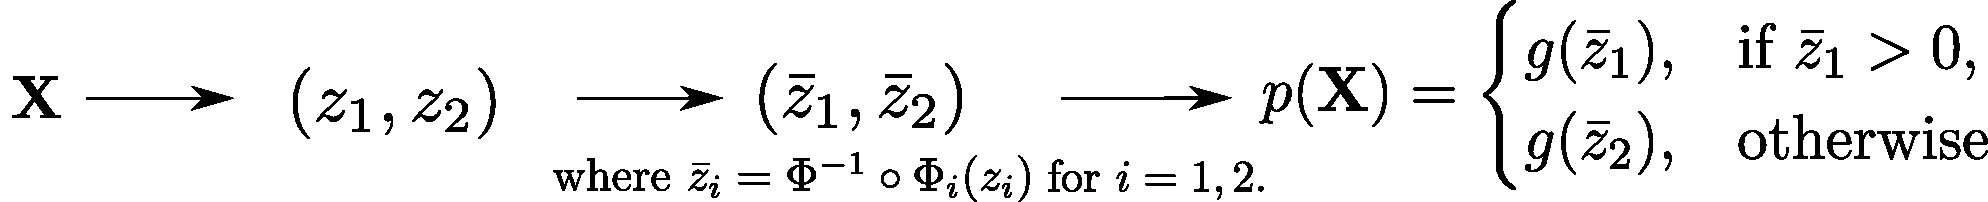
\includegraphics[width=.7\textwidth]{math.pdf}}
%\begin{equation}
%\mX \to (z_1,z_2) \to 
%(\bar z_1, \bar z_2)
%\to p(\mX)=
%\begin{cases}
%g(\bar z_1), & \text{if }\bar z_1>0,\\
%g(\bar z_2), & \text{otherwise}. 
%\end{cases}
%\end{equation}
We set $\Phi_i = $ empirical cumulative distribution function (CDF) of $z_i$ for $i=1,2$; $\Phi = $ CDF of standard normal; $g(z)=(1+\exp(z))^{-1}$; matrix dimension $d=20,30,\ldots,60$; and training sample size $n=100, 150, \ldots, 400$. The construction of $p$ amounts to a high nonlinearity from $\mX$ to $p(\mX)$. Unlike parametric methods, the functional form of $p$ is set unknown to the algorithm. 

\begin{figure}[H]
\centering
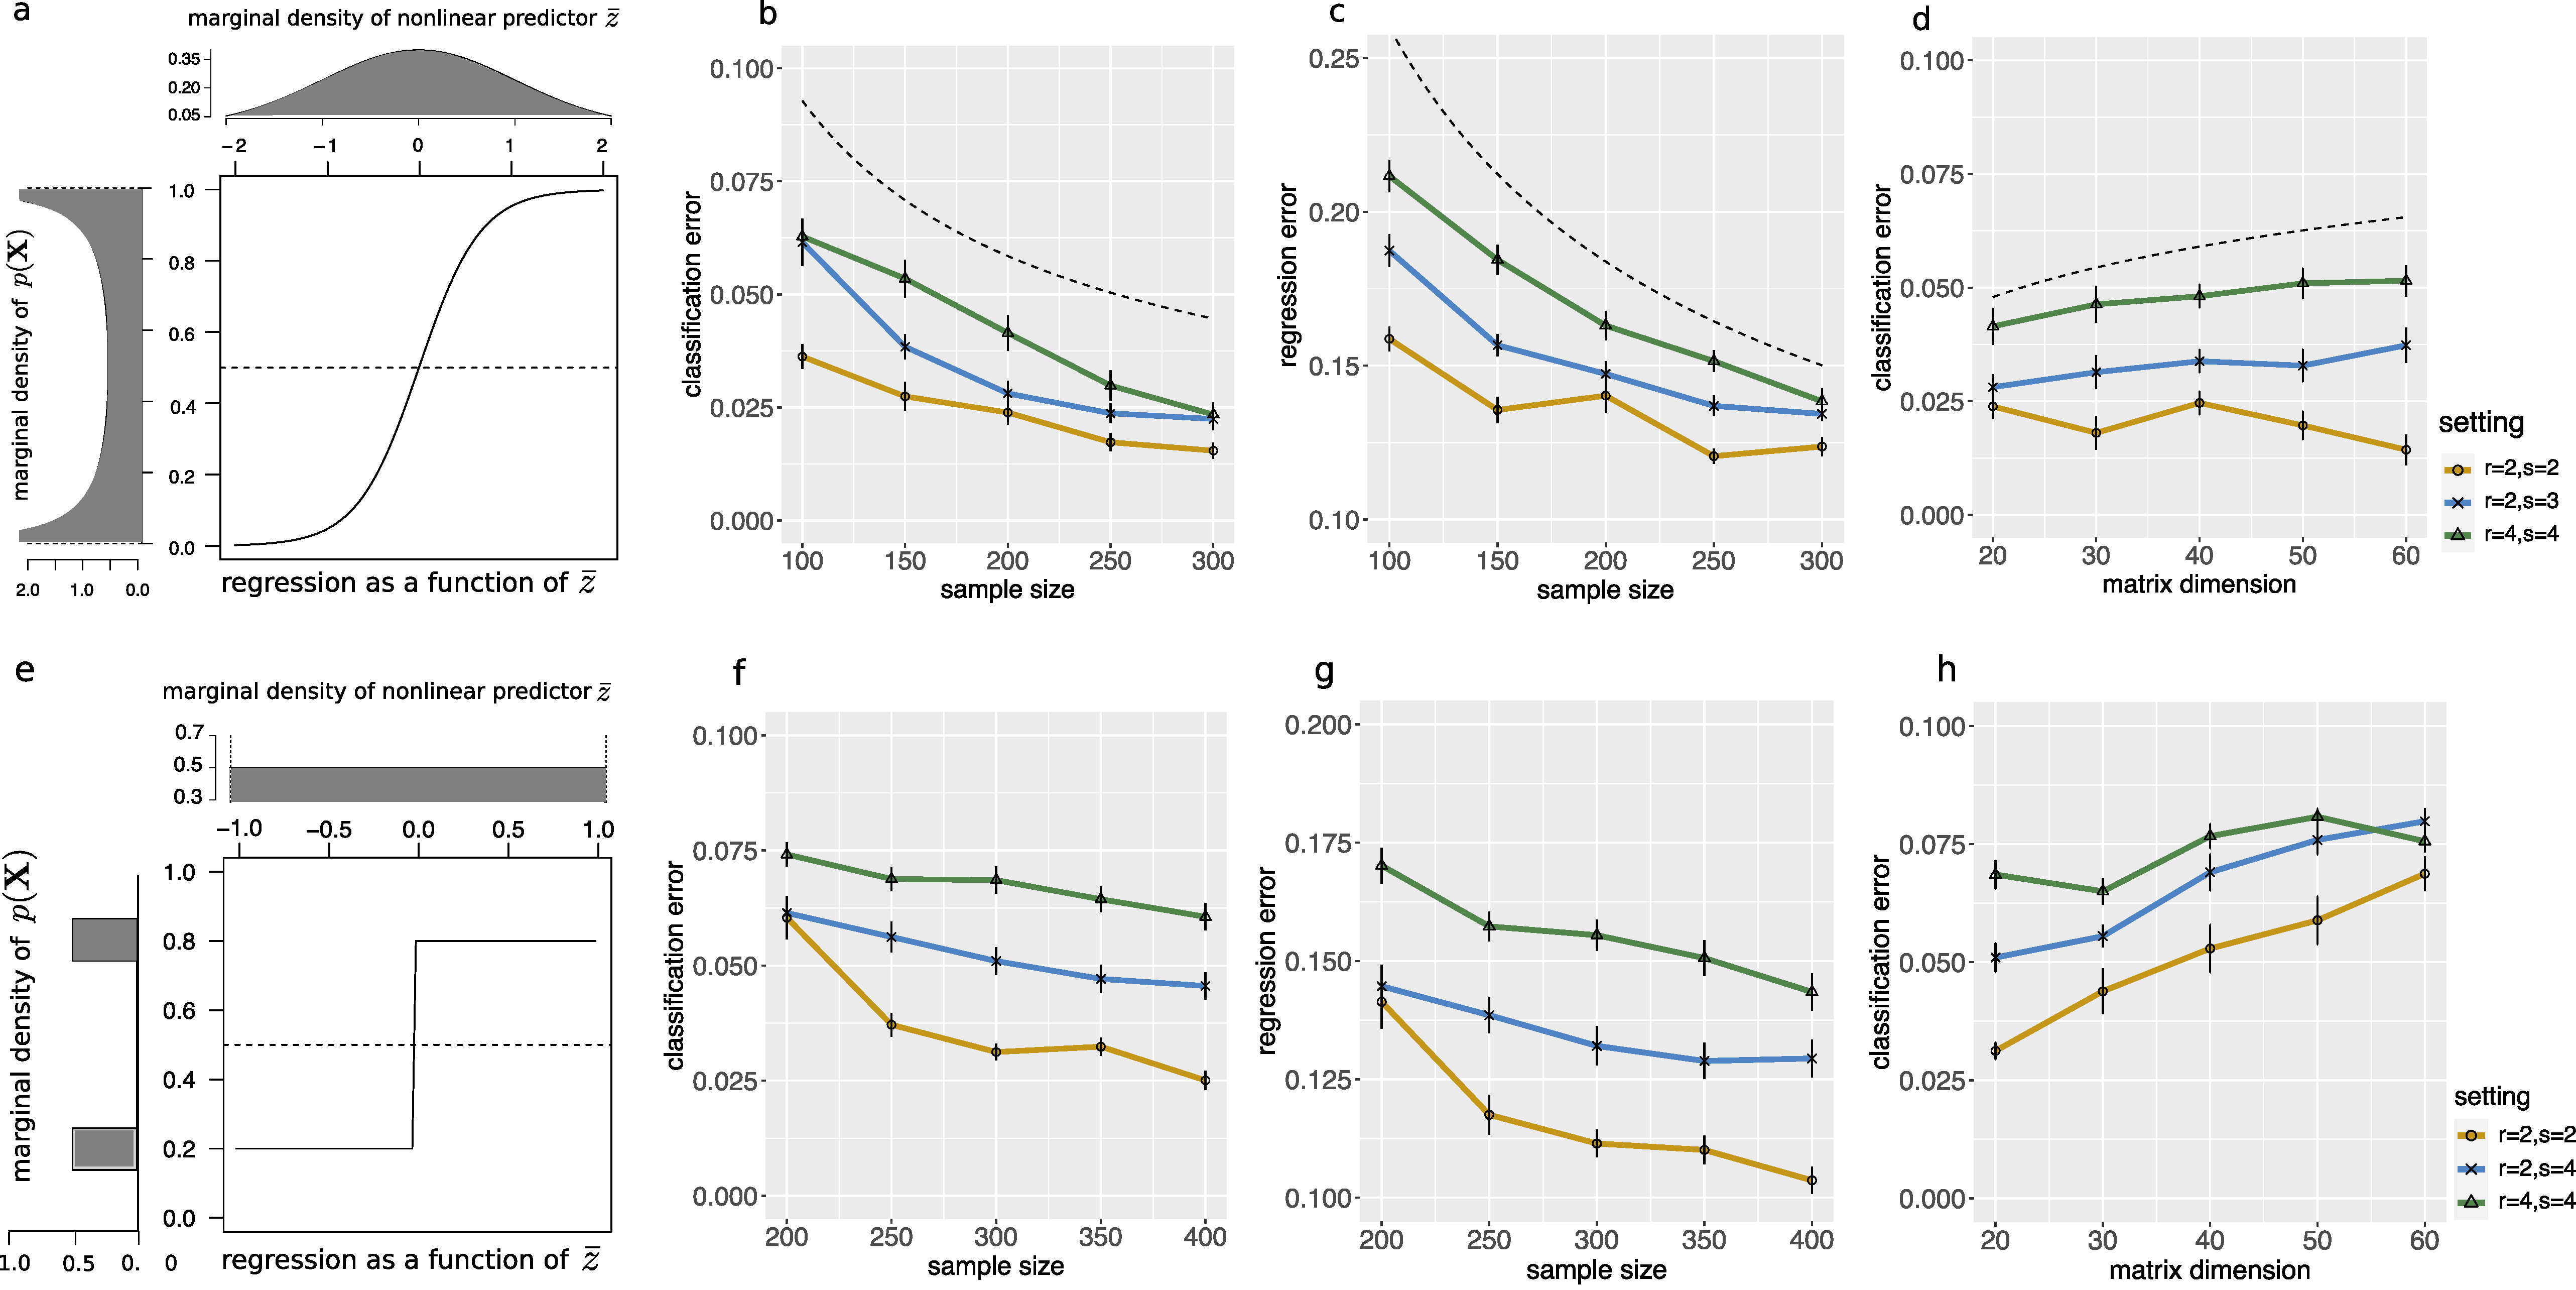
\includegraphics[width=1\textwidth]{combined.pdf}
\caption{Finite sample accuracy under two settings. Panels (a) and (e) summarize the simulation setup, panels (b, d) and (f, h) assess the performance in matrix classification, and panels (c, g) assess the matrix regression. }\label{fig:logistic}
\vspace{-.8cm}
\end{figure}

We first assess the prediction performance under model settings depicted in Figure~\ref{fig:logistic}a. 
Figures~\ref{fig:logistic}b-c show the polynomial decays of both classification and regression errors with respect to sample size, which is consistent with our theoretical results. We find that a higher rank or a denser coefficient leads to a higher error, as reflected by the upward shift of the curve as $(r,s)$ increases. Indeed, a higher $(r,s)$ implies a higher model complexity, thus increasing the generalization error. Figure~\ref{fig:logistic}d demonstrates that the error increases slowly with matrix dimension, and the growth appears well controlled by the log rate. The ability to effectively control massive noisy features highlights the benefit of our method in high dimensions. 

Figure~\ref{fig:logistic}e investigates a model setting that falls on the other end of the spectrum. The random variable $p(\mX)$ concentrates at two mass points $\pi=0.2$ and $0.8$. This makes the $\pi$-level set estimation challenging around $\pi=0.2$ and $0.8$, because of the nonidentifiability in the weighted classification. Interestingly, we find that our method maintains good performance on classification at $\pi=0.5$ (Figures~\ref{fig:logistic}f-h) and the overall regression (Figure~\ref{fig:logistic}g). The results demonstrate the robustness of our method against off-target level sets, as long as the majority are accurate.

Next, we compare our method {\bf \small Non}parametric {\bf \small MA}trix {\bf \small R}egression ({\bf \small NonMAR}) with several popular alternative methods: regular lasso ({\bf \small Lasso},~\cite{friedman2010regularization}), parametric regression for network predictors with group lasso ({\bf \small LogisticM},~\cite{relion2019network}), and convolutional neural network ({\bf \small CNN}). We choose a range of representative methods and investigate the benefit of each approach. The \Lasso serves as a baseline to assess the gain of matrix-valued predictors over vector-valued predictors. The methods \CNN and \NonparaM are nonparametric approaches and \LogisticM is a parametric solution for matrix based prediction.  
 \vspace{-.2cm}
\begin{figure}[ht]
    \centering
    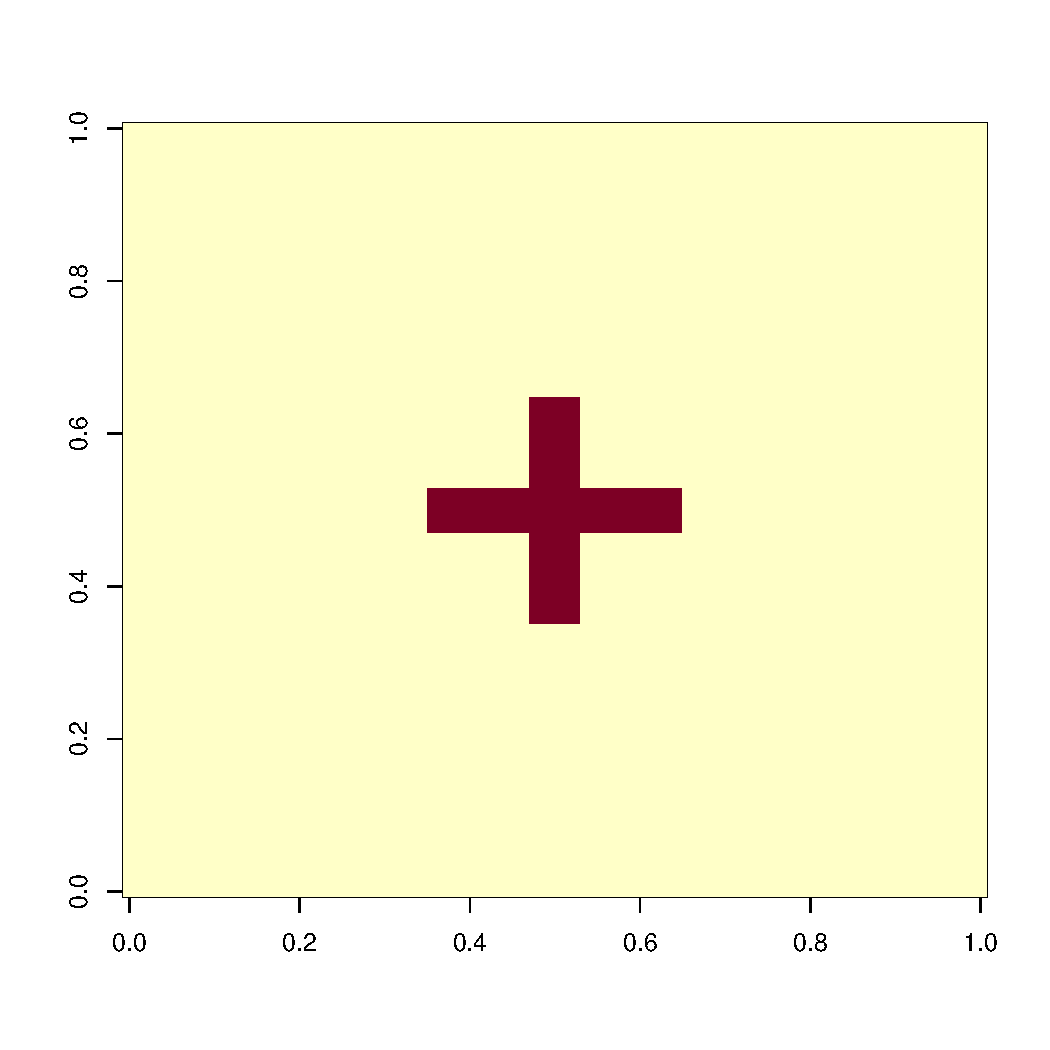
\includegraphics[width=3.8cm]{cross.pdf}
      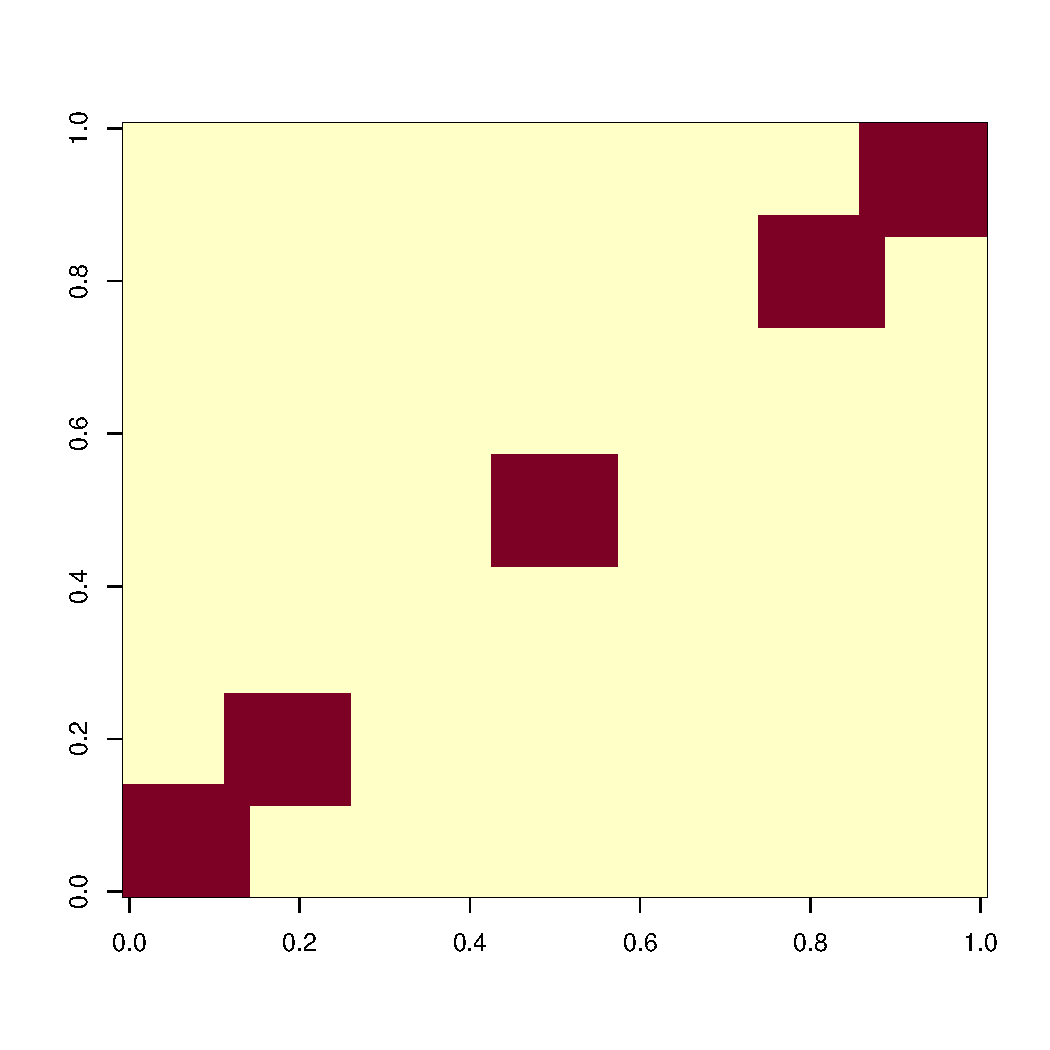
\includegraphics[width=3.8cm]{block.pdf}
        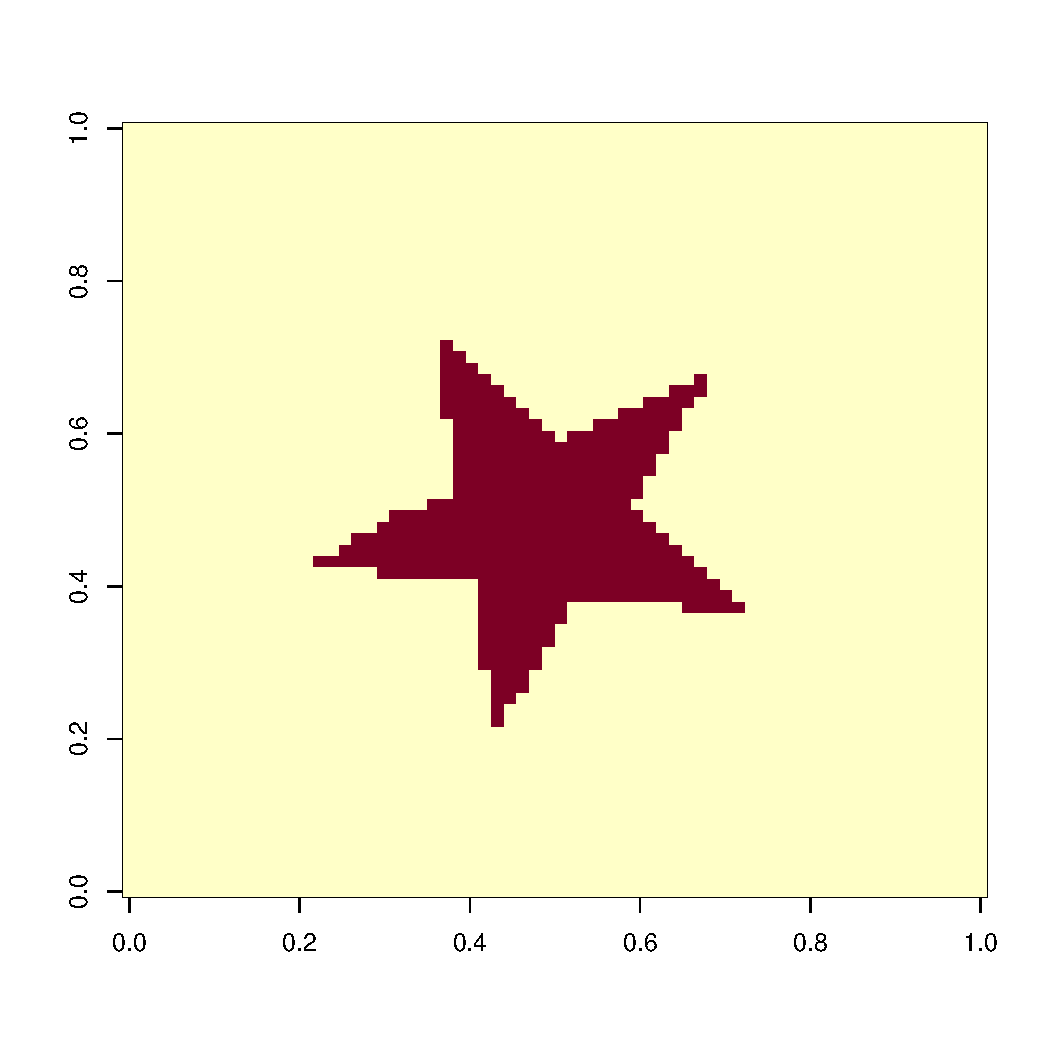
\includegraphics[width=3.8cm]{star.pdf}
          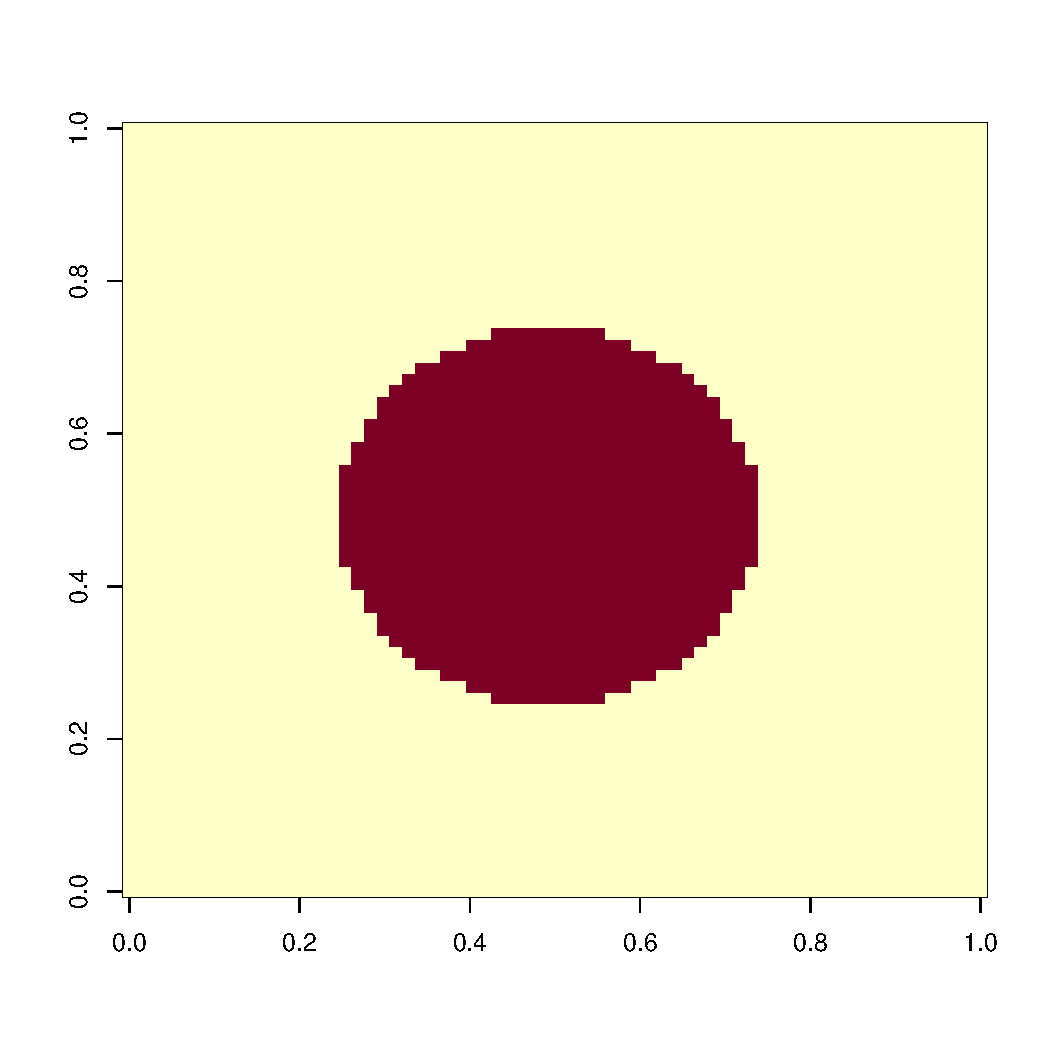
\includegraphics[width=4.7cm]{circle.pdf}
            
          \caption{Four active pattern in simulations. The active region is divided into four or five subregions (denoted I, II, ...), each of which has its own edge connectivity signal $g_{pq}(\pi)$.}\label{fig:region}
           \vspace{-.5cm}
\end{figure}

For fair comparison, we adopt similar simulation setup as in~\cite{relion2019network}, except that we add more challenging network patterns in order to assess model misspecification. We simulate the data $(\mX_i, y_i)_{i\in[n]}$ from latent variable model $(\mX,y)|\pi$ based on the following scheme,
\[
\pi \sim_{\text{i.i.d.}} \text{Uniform}[0,1] \stackrel{\text{conditional on $\pi$}}{\longrightarrow}
\begin{cases}
y\sim \text{Ber}(\pi),\ \text{}y\perp \mX|\pi, \\
\mX=\entry{\mX_{pq}}, \ \text{where\ } \mX_{pq}\sim_{\text{i.i.d.}} \tN(g_{pq}(\pi)\mathds{1}(\text{edge $(p,q)$ is active}), \sigma^2).
\end{cases}
\]
The edge connectivity signal, $g_{pq}(\pi)$, varies depending on the response probability $\pi$ and location of $(p,q)\in[d]^2$. Figure~\ref{fig:region} illustrates the active pattern which specifies the locations of active edges. The active region is further divided into several subregions, each of which has its own signal function $g_{pq}(\cdot)\colon [0,1]\to \mathbb{R}$. The function form of $g_{pq}(\cdot)$ is randomly drawn from a pre-specified library consisting of common functions such as $g(z)=\log(5z+1), 3\tan(z),6z^2,\ldots$.We set $d=68$, a training size $n=160$, and a test size $80$. The hyperparameters in all considered methods are selected by either default setting ({\bf \small LogisticM}) or cross validation ({\bf \small NonparaM}, {\bf \small Lasso}, {\small \bf CNN}). 


\begin{figure}[ht]
    \centering
    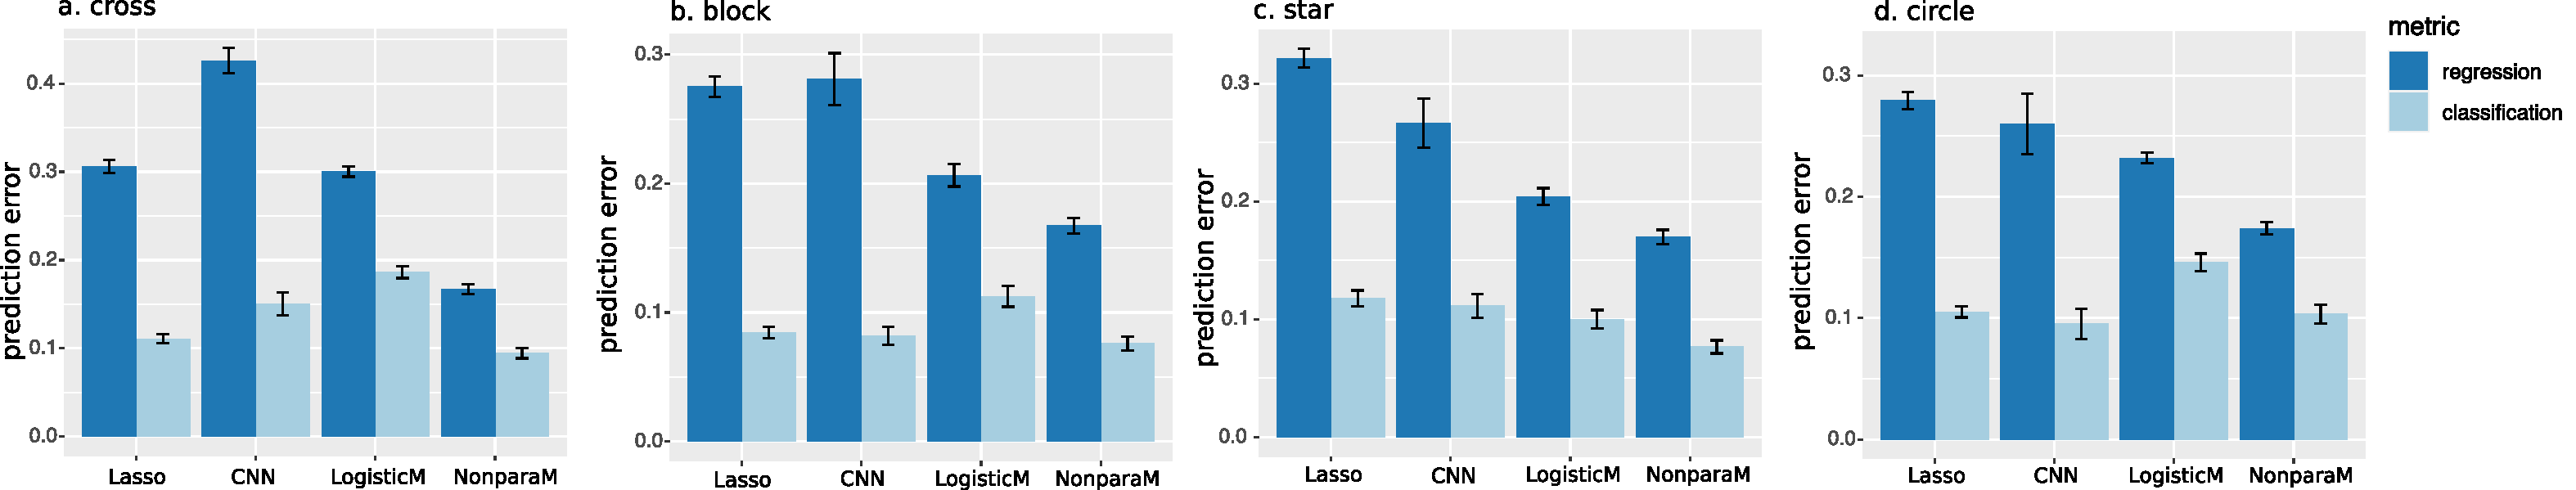
\includegraphics[width=\textwidth]{error_tot_comb2.pdf}
    \caption{Performance comparison between various methods under four different active patterns. }\label{fig:compare}
\end{figure}

Figure~\ref{fig:compare} compares the prediction accuracy between different methods. We find that {\bf \small NonMAR} consistently outperforms others, and the reduction in regression error is substantial. For example, the relative reduction in regression error using \NonparaM over the next best approach, {\bf \small LogisticM}, is over 20\% for patterns a and d, and over 15\% for patterns b and c. In contrast, neither \Lasso nor \CNN has satisfactory performance. One possible reason is that these two methods fail to appropriately incorporate the network structure of the predictors. The \Lasso takes vectorized matrices as inputs and therefore losses the two-way pairing information. On the other hand, \CNN assumes spacial ordering within row/column indices. Although local similarity is an appropriate model for common imaging analysis, the row/column indices are meaningless for networks. The only exception is the circle pattern where the \CNN has a lower classification error by a slight margin. This is perhaps due to the fact that circle pattern is nearly full rank which favors complicated models such as {\bf \small CNN}. Nevertheless, our method \NonparaM achieves stable performance in spite of its simplicity. 

\begin{figure}[ht]
    \centering
   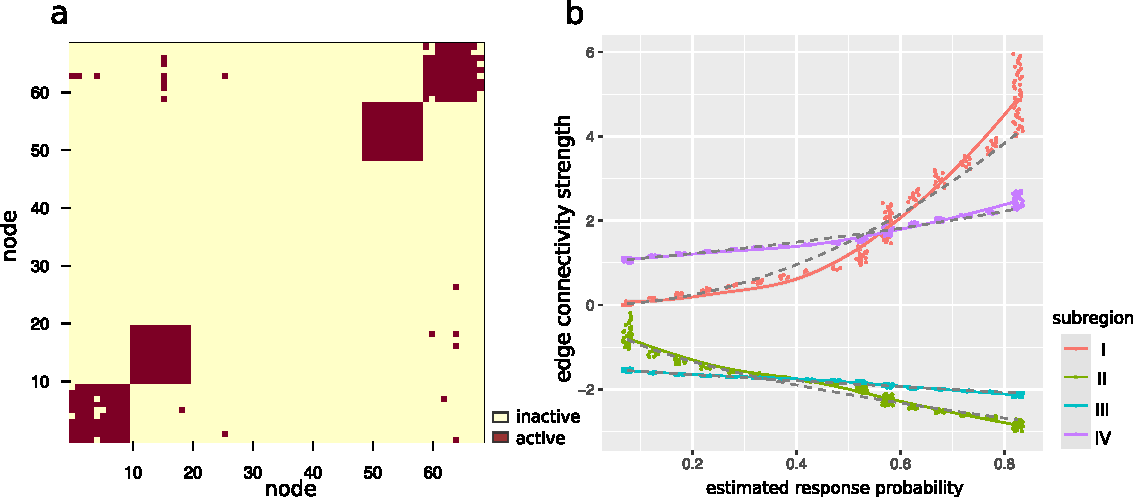
\includegraphics[width=8.4cm]{est_block.pdf}
          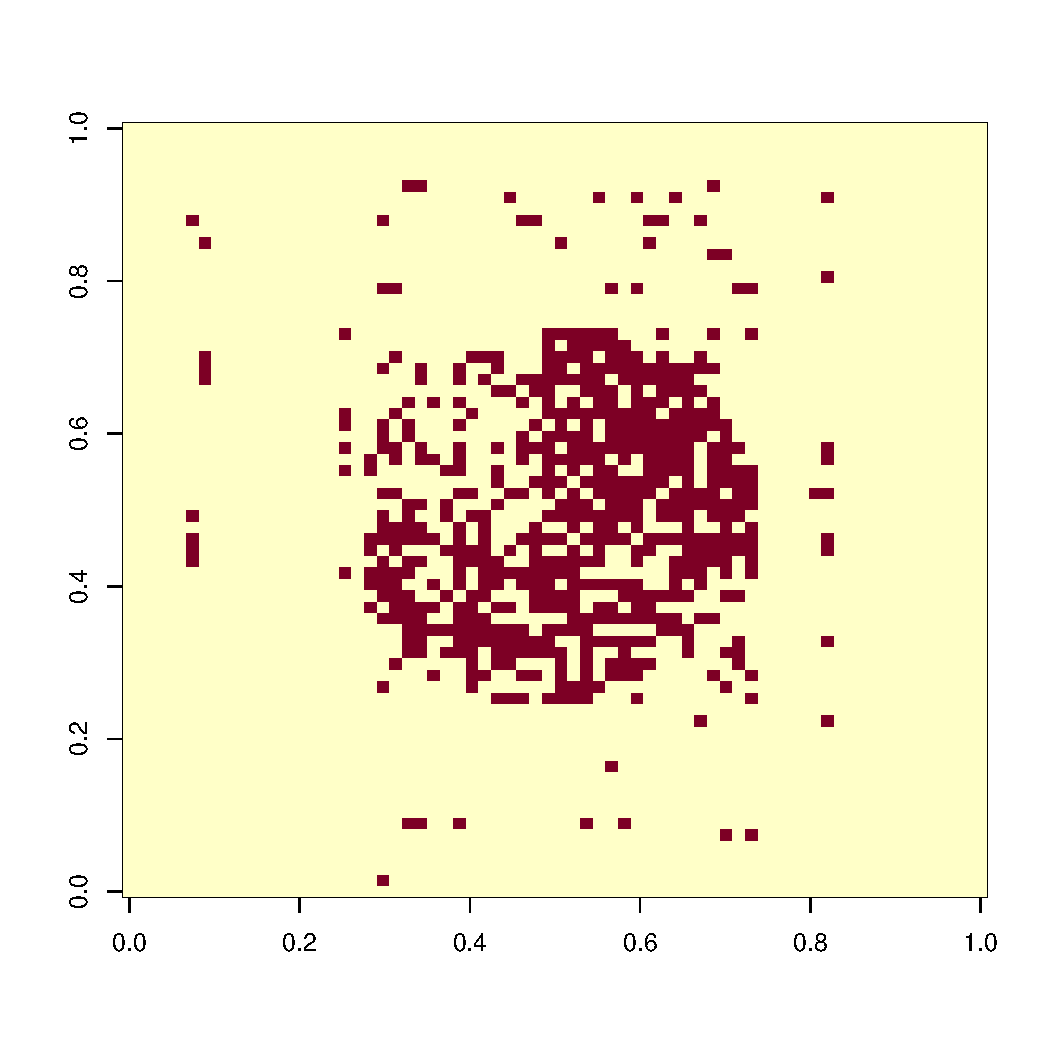
\includegraphics[width=8.4cm]{est_circle.pdf}
 \caption{Example outputs returned by {\bf \footnotesize NonMAR}. Panels (a) and (c) plot the top edges selected by our method. Panels (b) and (d) are scatter plots of the edge connectivity strength (averaged by subregion) versus the estimated response probability. The ground truth function is depicted in dashed curve.}\label{fig:compare2}
  \vspace{-.5cm}
\end{figure}


We provide illustrate examples to show the outputs returned by {\bf \small NonMAR}. Figures~\ref{fig:compare2}a and c plot the top edges selected by \NonparaM based on the moving averages of feature weights $(\hat \mB_\pi)_{\pi\in[0,1]}$ with a window size $\Delta \pi = 0.2$. The selected region agrees well with the ground truth (Figures~\ref{fig:compare}a and c). We also investigate the relationship between edge connectivity for individual $i$ and the estimated response probability $\hat \pi_i$. The trajectory of the edge connectivity accurately resembles the ground truth function in each subregion. The results demonstrate that our method is able to recover the right ``sorting'' of individuals with respect to the response probability on a continuous spectrum. 
The successful recovery of complicated unknown functions makes our method {\bf \small NonMAR} appealing in applications. 

\vspace{-.3cm}
\section{Application to human brain connectome data}
\vspace{-.5cm}

We apply our method to brain network data from Human Connectome Project (HCP). We analyze the Variable Short Penn Line Orientation Test (VSPLOT) score which measures the individual's visuospatial processing ability. We preprocess the data as in~\cite{wang2019common}, and analyze $n=212$ individuals whose VSPLOT scores are either high ($y=1$) or low ($y=-1$). Each individual's brain network is represented by a 68-by-68 binary adjacency matrix $\mX\in\{0,1\}^{68\times 68}$, with the entries encoding the presence or absence of fiber connections between the 68 brain nodes. We adjust age and gender as additional covariates in the prediction, and use a random 60-20-20 split of the data for training, validation, and testing. 

\begin{figure}[H]
    \centering
       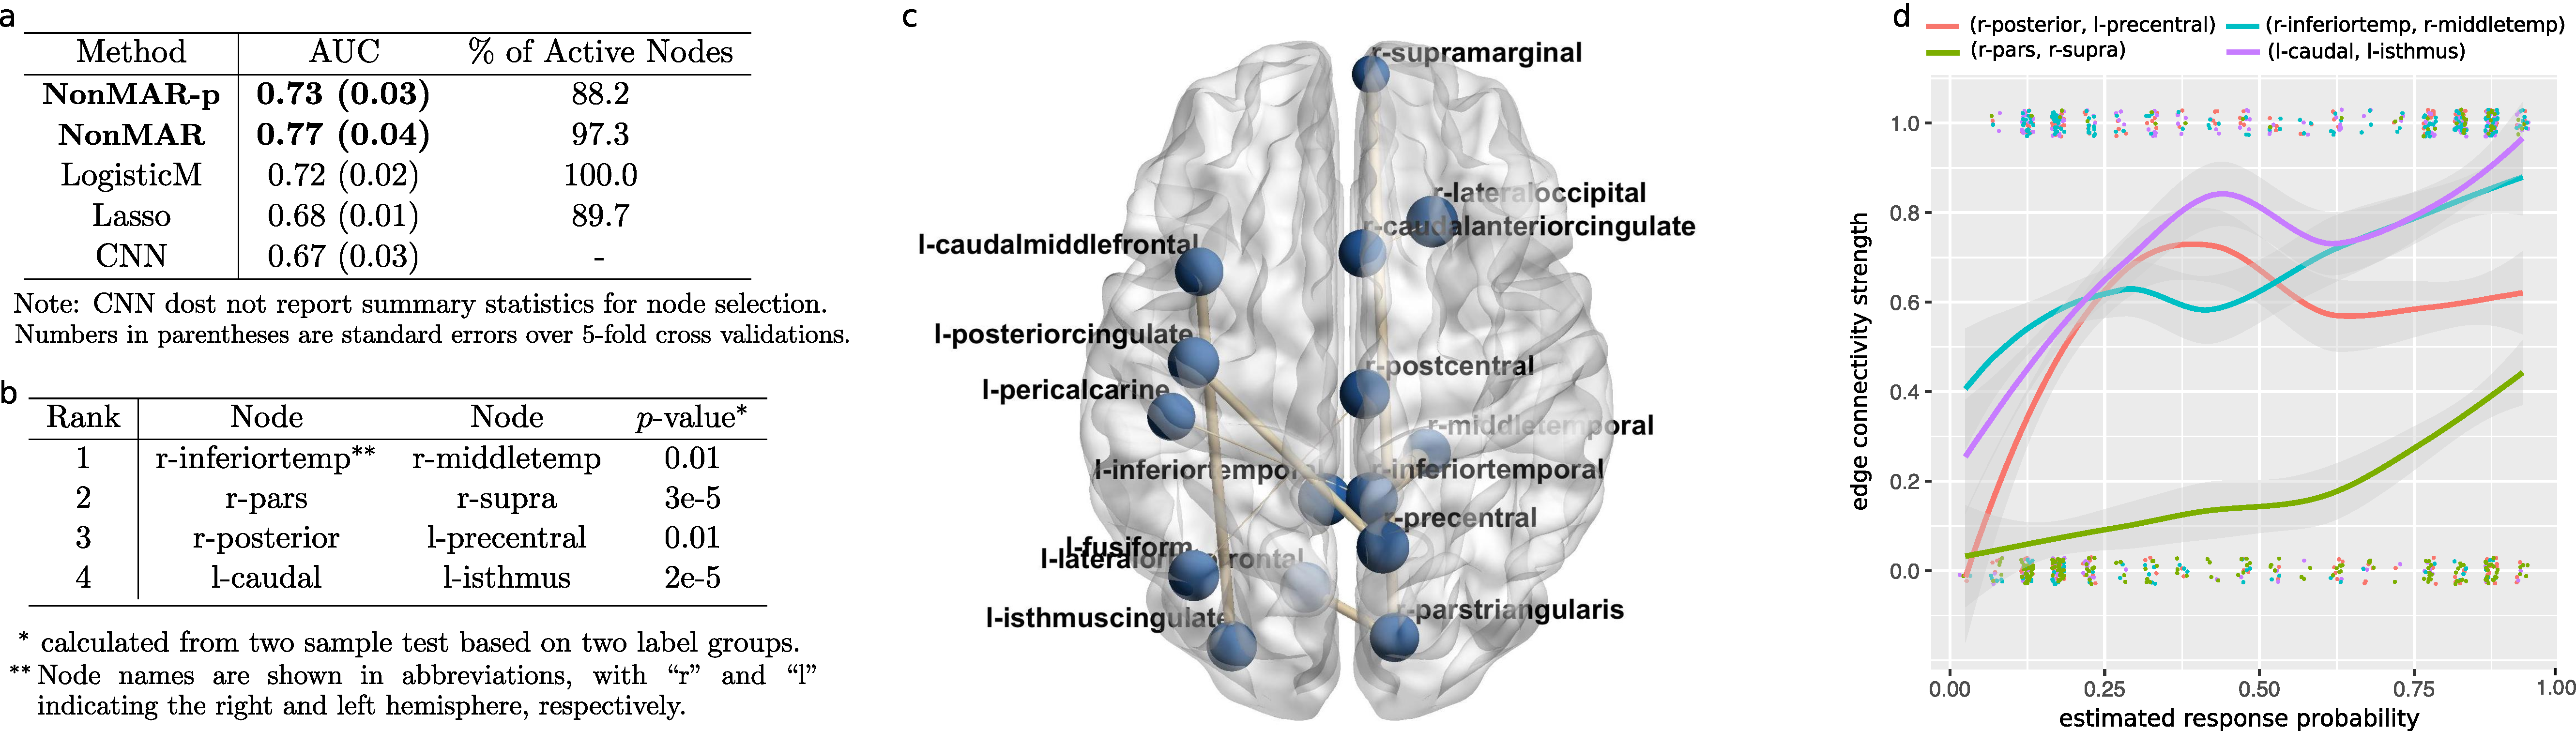
\includegraphics[width=\textwidth]{HCP_combined.pdf}
 \caption{HCP analysis results. (a) Comparison of prediction accuracy. (b) Top edges selected by our method {\scriptsize \bf NonMAR-p}. (c) Top edges overlaid on brain template. (d) Edge connectivity strength versus estimated response probability. Colored curves represent the moving averages of connectivity strengths, gray bands represent one standard error, and jitter points represent the raw connectivity values (0 or 1). }\label{fig:real}
 \vspace{-.7cm}
\end{figure}

We compare our performance to other methods using the same procedure as in the previous section. Figure~\ref{fig:real}a shows that our method achieves high regression accuracy, measured by area under receiver operating characteristic (AUC). As common in high-dimensional settings, we observe that models with optimal cross-validation accuracy tend to include many noise variables. A useful heuristic is the so-called ``one-standard-error rule''~\citep{hastie2015statistical}, in which one selects the most parsimonious model with cross-validation accuracy within one standard error of the best. We apply this rule and report the results as {\bf \small NonMAR-p}. It is remarkable to see that {\bf \small NonMAR-p} results in 12\% reduction of active nodes but still achieves excellent accuracy (AUC = 0.73). 



Figure~\ref{fig:real}b lists the top brain edges identified by our method. Edges are ranked by their maximal values in the feature weights $(\hat \mB_\pi)_{\pi \in [0,1]}$ via moving averaging. We find that the top edges involve connections between frontal and occipital regions in the right hemisphere. This seems consistent with recent evidence of dysfunction in right posterior regions for deficits in visuospatial processing~\citep{wang2019common}. We also find nonlinear relationship between edge connection strength and response probability. For example, the connection (r-parstriangularis, r-supramarginal) grows slowly when $\pi$ is low but fast when $\pi$ is high. In contrary, the connection (r-posteriorcingulate, r-precentral) grows fast initially and then reaches a plateau as $\pi$ increaases. The detected pattern reveals the heterogeneous changes in brain connectivities with respect to visuospatial processing ability. 

\vspace{-.3cm}
\section{Conclusion}
\vspace{-.5cm}
We have developed a nonparametric framework for learning the relationship between a binary label response and a high-dimensional matrix-valued predictor. 
Theoretical and numerical results demonstrate the advantages of our method. Our work unlocks several open directions. Extension to multilclass probability estimation and to nonlinear boundaries would be of future interest. 

\singlespacing
\bibliographystyle{chicago}

\bibliography{tensor_wang}



\end{document}



